\documentclass{article}
\usepackage{multicol}
\usepackage{xcolor}
\usepackage{graphicx}
\linespread{1.35}
\usepackage{amsmath}
\usepackage{color}
\usepackage{tikz}
\usetikzlibrary{arrows,automata}

\begin{document}

\begin{flushright}
 \texttt{Finite Automata} \hspace*{0.1cm}\textbf{$|$} \hspace*{0.1cm} \textbf{117}\hspace*{0.1cm}
\end{flushright}
\vspace*{0.5cm}

26. Prove that the following two FA are equivalent.

\begin{center}
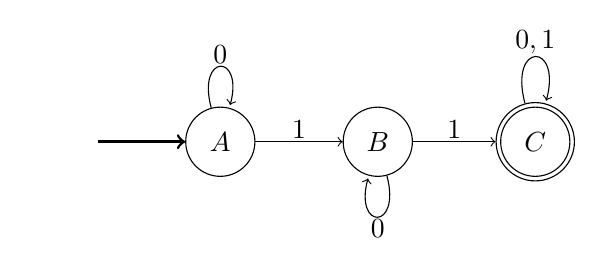
\begin{tikzpicture}[node distance = 2cm,auto,inner sep=1pt]
\node[state,draw=white,inner sep=0pt] (A) {$$};
\node[state,draw=black] (B) [ right of = A]  {$A$};
\node[state,draw=black] (C) [right of = B]  {$B$};
\node[state,draw=black,inner sep=10pt] (D) [right of = C]  {$$};
\node[state,draw=black] (E) [right of = C]  {$C$};

\path (A) edge [->,line width=1pt,node distance = 0.1cm] node {$$} (B);
\path (B) edge [->,loop above] node {$0$} (B);
\path (D) edge [->,loop above] node {$0,1$} (D);
\path (B) edge [->] node {$1$} (C);
\path (C) edge [->] node {$1$} (D);
\path (C) edge [->,loop below] node {$0$} (B);

\end{tikzpicture}
\end{center}

\begin{center}
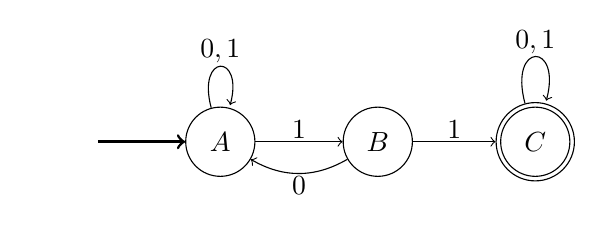
\begin{tikzpicture}[node distance = 2cm,auto,inner sep=1pt]
\node[state,draw=white,inner sep=0pt] (A) {$$};
\node[state,draw=black] (B) [ right of = A]  {$A$};
\node[state,draw=black] (C) [right of = B]  {$B$};
\node[state,draw=black,inner sep=10pt] (D) [right of = C]  {$$};
\node[state,draw=black] (E) [right of = C]  {$C$};

\path (A) edge [->,line width=1pt,node distance = 0.1cm] node {$$} (B);
\path (B) edge [->,loop above] node {$0,1$} (B);
\path (D) edge [->,loop above] node {$0,1$} (D);
\path (B) edge [->] node {$1$} (C);
\path (C) edge [->] node {$1$} (D);
\path (C) edge [->,bend left =30]  node {$0$} (B);

\end{tikzpicture}
\end{center}

\textbf{Solution:} The second one is an NFA. The tabular representation of the FA is

\vspace*{0.4cm}
\begin{center}
\begin{tabular}{ccc}
 \hline

 \hline

 \hline

 \hline
 & \multicolumn{2}{c}{$Next State$}\\
 \cline{2-3}
 $Present State$ &  $i=0$ & $i=1$\\
\hline
 $A$   &   $A$      &  $A,B$ \\
 $B$   &   $-$      &  $C$   \\
 $C$   &   $C$      &  $C$   \\
 \hline

 \hline

 \hline

 \hline
\end{tabular}
\end{center}

The DFA from the given NFA is

\vspace*{0.4cm}
\begin{center}
\begin{tabular}{ccc}
 \hline

 \hline

 \hline

 \hline
 & \multicolumn{2}{c}{$Next State$}\\
 \cline{2-3}
 $Present State$ &  $i=0$ & $i=1$\\
\hline
     $[A]$     &    $[A]$   &    $[A, B]$  \\
   $[A, B]$    &    $[A]$   &  $[A, B, C]$ \\
 $[A, B, C]$   &  $[A, C]$  &   $[B, C]$   \\
  $[B, C]$     &  $[B, C]$  &   $[B, C]$   \\
 $[B, C]$      &  $[A, C]$  &    $[C]$    \\
  $[C]$        &   $[C]$    &    $[C]$    \\

\end{tabular}
\end{center}

Simplifying this, the DFA becomes

\begin{center}
\begin{tabular}{ccc}
 \hline

 \hline

 \hline

 \hline
 & \multicolumn{2}{c}{$Next State$}\\
 \cline{2-3}
 $Present State$ &  $i=0$ & $i=1$\\
\hline
 $S_1$   &   $S_1$      &  $S_2$ \\
 $S_2$   &   $S_1$      &  $S_3$   \\
 $S_3$   &   $S_4$      &  $S_5$   \\
 $S_4$   &   $S_5$      &  $S_5$   \\
 $S_5$   &   $S_4$      &  $S_6$  \\
 $S_6$   &   $S_6$      &  $S_6$  \\
 \hline

 \hline

 \hline

 \hline
\end{tabular}
\end{center}


Here, $S_1$ is the initial and $S_3$, $S_4$, $S_5$, and $S_6$ are the final states.\\
 \hspace*{0.5cm} Now try to minimize the DFA.
 \begin{center}
   $P_0 = (S_1 S_2 S_3 S_4 S_5 S_6)$\\
   $P_1 = (S_1 S_2)(S_3 S_4 S_5 S_6)$\\
   $P_2 = (S_1) (S_2) (S_3 S_4 S_5 S_6)$\\
 \end{center}
 
 \begin{flushleft}
    \textbf{118}\hspace*{0.1cm} \textbf{$|$} \hspace*{0.1cm} \texttt{Introduction to Automata Theory, Formal Languages and Computation}
  \end{flushleft}
  \vspace*{0.5cm}

  Rename $(S_1)$ as $A, (S_2)$ as $B$, and $(S_3 S_4 S_5 S_6)$ as $C$. The minimized $FA$ is\\

  \vspace*{0.2cm}
  \begin{center}
\begin{tabular}{ccc}
 \hline

 \hline

 \hline

 \hline
 & \multicolumn{2}{c}{$Next State$}\\
 \cline{2-3}
 $Present State$ &  $i=0$ & $i=1$\\
\hline
 $A$   &   $A$      &  $B$ \\
 $B$   &   $A$      &  $C$   \\
 $C$   &   $C$      &  $C$   \\
 \hline

 \hline

 \hline

 \hline
\end{tabular}
\end{center}

\vspace*{0.2cm}
where A is the initial state and C is the final state.\\
 \hspace*{0.5cm} It is proved that the two DFA are equivalent.\\
 
 27. Draw the state transition of a deterministic finite state automaton which accepts all strings from
the alphabet (a, b), such that no string has three consecutive occurrences of the letter b.\\
\begin{flushright}
  [GATE 1993]
\end{flushright}


\textbf{Solution:}\\

\begin{center}
\section{picture}
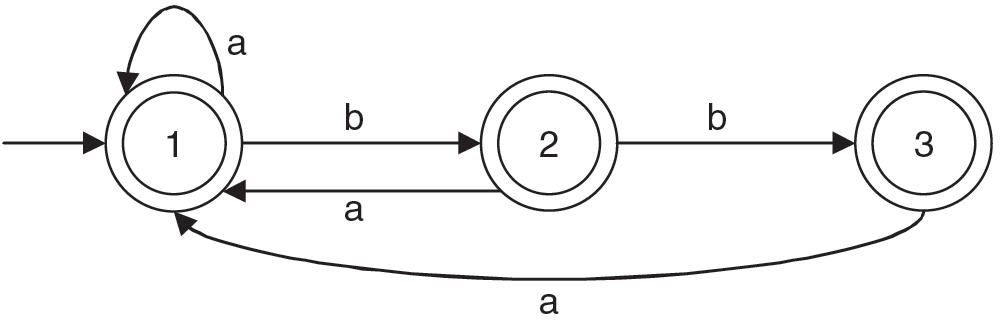
\includegraphics[width=7cm,height=2.5cm]{118.png}
\end{center}


28. Construct a finite state machine with minimum number of states, accepting all strings over (a, b)
such that the number of a' s is divisible by two and the number of b's is divisible by three.\\
\begin{flushright}
  [GATE 1997]
\end{flushright}


\textbf{Solution:}\\
\begin{center}
\section{picture}
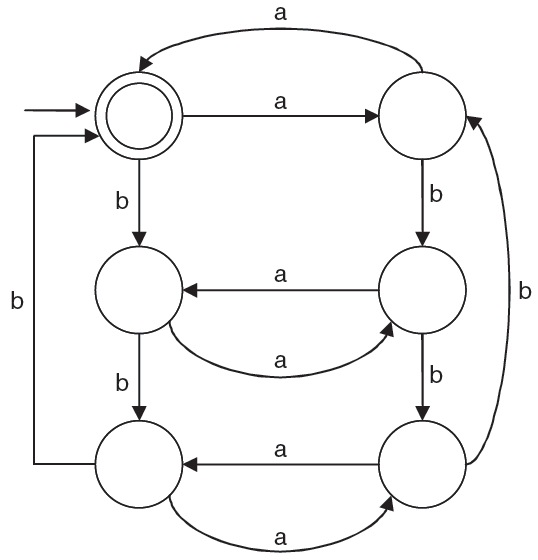
\includegraphics[width=5cm,height=5cm]{118-2.png}
\end{center}

\begin{flushright}
 \texttt{Finite Automata} \hspace*{0.1cm}\textbf{$|$} \hspace*{0.1cm} \textbf{119}\hspace*{0.1cm}
\end{flushright}


\begin{center}
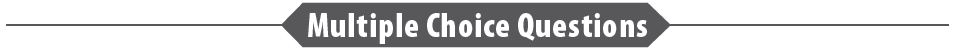
\includegraphics[width=11cm,height=0.7cm]{119.png}
\end{center}


1. A language L from a grammar $G = \{V_N, \Sigma,P, S\}$ is\\
\hspace*{0.5cm} a) Set of symbols over $V_N$ \\
\hspace*{0.5cm} b) Set of symbols over $\Sigma$ \\
\hspace*{0.5cm} c) Set of symbols over $P$ \\
\hspace*{0.5cm} d) Set of symbols over $S$ \\

\vspace*{0.2cm}
2. Which is true for $\delta(q, ab)$ \\
\hspace*{0.5cm} a) $\delta(q, a) \cup \delta(q, b)$ \\
\hspace*{0.5cm} b) $\delta(\delta(q, a), b)$ \\
\hspace*{0.5cm} c) $\delta(q, a), b$ \\
\hspace*{0.5cm} d) $\delta(q, a) \cap \delta(q, b)$ \\

\vspace*{0.2cm}
3. The transitional function of a DFA is\\
\hspace*{0.5cm} a) $Q \times \Sigma \rightarrow Q$    \hspace*{0.7cm}  b) $Q \times \Sigma \rightarrow 2^Q$\\
\hspace*{0.5cm} c) $Q \times \Sigma \rightarrow 2^n$  \hspace*{0.7cm}  d) $Q \times \Sigma \rightarrow Q^n$\\


\vspace*{0.2cm}
4. The transitional function of an NFA is \\
\hspace*{0.5cm} a) $Q \times \Sigma \rightarrow Q$      \hspace*{0.7cm} b) $Q \times \Sigma \rightarrow 2^Q$ \\
\hspace*{0.5cm} c) $Q \times \Sigma \rightarrow 2^n$    \hspace*{0.7cm} d) $Q \times \Sigma \rightarrow Q^n$ \\


\vspace*{0.2cm}
5. The maximum number of states of a DFA converted from an NFA with n states is \\
\hspace*{0.5cm} a) n          \hspace*{0.7cm}    b) $n^2$ \\
\hspace*{0.5cm} c) $2^n$    \hspace*{0.7cm}    d) None of these \\

\vspace*{0.2cm}
6. A string after full traversal is called not accepted by an NFA if it results in\\
\hspace*{0.5cm} a) Some non-final states\\
\hspace*{0.5cm} b) All non-final states\\
\hspace*{0.5cm} c) A single non-final state \\
\hspace*{0.5cm} d) Some final states \\

\vspace*{0.2cm}

7. An NFA with a set of states $Q$ is converted to an equivalent DFA with a set of states $Q'$. Find which is true.\\
\hspace*{0.5cm} a) $Q' = Q$             \hspace*{0.7cm}     b) $Q' \subseteq Q$ \\
\hspace*{0.5cm} c) $Q \subseteq Q'$        \hspace*{0.7cm}  d) None of these \\

\vspace*{0.2cm}
8. The basic limitations of a finite state machine is \\
\hspace*{0.5cm} a) It cannot remember arbitrarily large amount of information \\
\hspace*{0.5cm} b) It cannot remember state transitions \\
\hspace*{0.5cm} c) It cannot remember grammar for a language \\
\hspace*{0.5cm} d) It cannot remember language generated from a grammar \\

\vspace*{0.2cm}
9. The string $WW^R$ is not recognized by any FSM because \\
\hspace*{0.5cm} a) An FSM cannot remember arbitrarily large amount of information\\
\hspace*{0.5cm} b) An FSM cannot fix the mid-point \\
\hspace*{0.5cm} c) An FSM cannot match W with $W^R$ \\
\hspace*{0.5cm} d) An FSM cannot remember the first and last inputs.\\

\vspace*{0.2cm}
10. A finite automata recognizes\\
\hspace*{0.5cm} a) Any language\\
\hspace*{0.5cm} b) Context sensitive language \\
\hspace*{0.5cm} c) Context-free language \\
\hspace*{0.5cm} d) Regular language \\

\vspace*{0.2cm}

11. Which is true for a dead state?\\
\hspace*{0.5cm} a) It cannot be reached anytime \\
\hspace*{0.5cm} b) There is no necessity of the state \\
\hspace*{0.5cm} c) If control enters, there is no way to come out from the state \\
\hspace*{0.5cm} d) If control enters, FA is dead \\

\vspace*{0.2cm}
12. The language accepted by the given FA is\\
\begin{center}
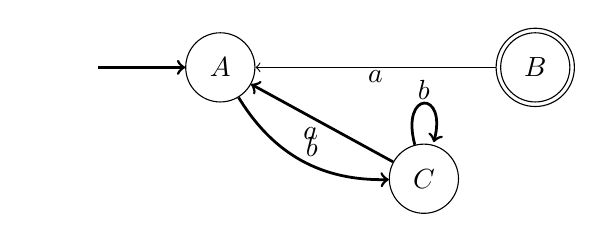
\begin{tikzpicture}[node distance = 2cm,auto,inner sep=1pt]
\node[state,draw=white,inner sep=0pt] (A) {$$};
\node[state,draw=black] (B) [ right of = A]  {$A$};
\node[state,draw=black,node distance = 4cm] (C) [right of = B]  {$B$};
\node[state,draw=black,inner sep=10pt,node distance = 4cm] (D) [right of = B]  {$$};
\node[state,draw=black] (E) [below left of = C]  {$C$};

\path (A) edge [->,line width=1pt,node distance = 0cm] node {$$} (B);
\path (D) edge [->] node {$a$} (B);
\path (E) edge [->,loop above,line width=1pt] node {$b$} (E);
\path (E) edge [->,line width=1pt] node {$a$} (B);
\path (B) edge [->,bend right,line width=1pt]  node {$b$} (E);

\end{tikzpicture}
\end{center}
\hspace*{0.5cm} a) $(ab)*$        \hspace*{0.7cm}  b) $bb*a$  \\
\hspace*{0.5cm} c) $b(ba)*a$      \hspace*{0.7cm}  d) Null \\

\vspace*{0.2cm}
13. In the previous FA, B is called\\
\hspace*{0.5cm} a) Dead state \\
\hspace*{0.5cm} b) Inaccessible state \\
\hspace*{0.5cm} c) Both a and b \\
\hspace*{0.5cm} d) None of these \\

\vspace*{0.2cm}

14. Which is true for a Moore machine?\\
\hspace*{0.5cm} a) Output depends on the present state \\
\hspace*{0.5cm} b) Output depends on the present input \\
\hspace*{0.5cm} c) Output depends on the present state and the present input \\
\hspace*{0.5cm} d) Output depends on the present state and the past input \\

\begin{flushleft}
    \textbf{120}\hspace*{0.1cm} \textbf{$|$} \hspace*{0.1cm} \texttt{Introduction to Automata Theory, Formal Languages and Computation}
  \end{flushleft}

\vspace*{0.3cm}
15. Which is true for the Mealy machine?\\
\hspace*{0.5cm} a) Output depends on the present state \\
\hspace*{0.5cm} b) Output depends on the present input \\
\hspace*{0.5cm} c) Output depends on the present state and the present input\\
\hspace*{0.5cm} d) Output depends on the present state and the past input\\

\vspace*{0.2cm}

16. Which is true for the inaccessible state?\\
\hspace*{0.5cm} a) It cannot be reached anytime \\
\hspace*{0.5cm} b) There is no necessity of the state \\
\hspace*{0.5cm} c) If control enters, there is no way to come out from the state \\
\hspace*{0.5cm} d) If control enters, FA is dead \\

\vspace*{0.2cm}
17. In Mealy Machine, O/P is a function of \\
\hspace*{0.5cm} a) Present state only\\
\hspace*{0.5cm} b) Next state only\\
\hspace*{0.5cm} c) Present state and Input\\
\hspace*{0.5cm} d) Input only\\

\vspace*{0.2cm}
18. In Moore Machine, O/P is associated with \\
\hspace*{0.5cm} a) Present state only \\
\hspace*{0.5cm} b) Next state only \\
\hspace*{0.5cm} c) Present state and Input \\
\hspace*{0.5cm} d) Input only \\

\vspace*{0.2cm}
19. Which type of string is accepted by the following finite automata? \\
\begin{center}
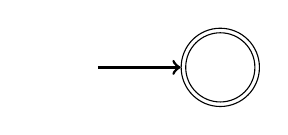
\begin{tikzpicture}[node distance = 2cm,auto,inner sep=1pt]
\node[state,draw=white,inner sep=0pt] (A) {$$};
\node[state,draw=black] (C) [right of = A]  {$$};
\node[state,draw=black,inner sep=10pt] (D) [right of = A]  {$$};

\path (A) edge [->,line width=1pt,node distance = 0cm] node {$$} (D);
\end{tikzpicture}
\end{center}

\hspace*{0.5cm} a) All string \\
\hspace*{0.5cm} b) Null string \\
\hspace*{0.5cm} c) No string \\
\hspace*{0.5cm} d) All of the above \\

\vspace*{0.2cm}

$Answers:$ \\
1. b    \hspace*{0.3cm}    2. b    \hspace*{0.3cm}   3. a     \hspace*{0.3cm}    4. b     \hspace*{0.3cm}    5. c     \hspace*{0.3cm}     6. b     \hspace*{0.3cm}     7. d       \hspace*{0.3cm}       8. a      \hspace*{0.3cm}    9. b      \hspace*{0.3cm}     10. d \\
11. c    \hspace*{0.3cm}    12. d     \hspace*{0.3cm}    13. b      \hspace*{0.3cm}    14. a      \hspace*{0.3cm}    15. c    \hspace*{0.3cm}     16. a     \hspace*{0.3cm}    17. b      \hspace*{0.3cm}       18. a     \hspace*{0.3cm}    19. b \\ 

\begin{center}
\section{picture}
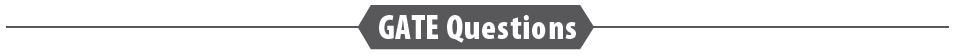
\includegraphics[width=11cm,height=0.7cm]{120.png}
\end{center}

1. Consider the strings $u = abbaba$, $v = bab$, and $w = aabb$. Which of the following statement is true
for the given transitional system?\\
\begin{center}
\section{picture}
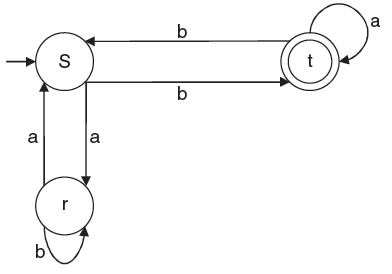
\includegraphics[width=4cm,height=3cm]{120-1.png}
\end{center}

\vspace*{0.1cm}
a) The automaton accepts u and v but not w.\\
b) The automaton accepts each of u, v, and w.\\
c) The automaton rejects each of u, v, and w.\\
d) The automaton accepts u but rejects v and w.\\

\end{document} 